\documentclass[a4paper,11pt]{report}

\usepackage{fullpage}

\usepackage{amsmath}
\usepackage{bussproofs}
\usepackage{mathpartir}
\usepackage{prooftrees}
\usepackage{placeins}
\usepackage{color}

% Minted
\usepackage[cache=false]{minted}

\newmintinline{c}{
  fontsize=\small,
  breaklines=true
}

\newminted{c}{
  frame=single,
  framesep=2mm,
  fontsize=\scriptsize,
  mathescape
}

\newminted[clinecode]{c}{
  frame=single,
  framesep=2mm,
  fontsize=\scriptsize,
  mathescape,
  linenos
}

\newcommand*{\BBox}[1]{\draw (#1 + 0.5,0.5) -- (#1 + 1.5,0.5) -- (#1 + 1.5,-0.2)
  -- (#1 + 0.5,-0.2) -- cycle;}
\newcommand*{\SBox}[1]{}

\newcommand*{\equal}{=}

% for finite state automata
\usepackage{tikz}
\usetikzlibrary{automata,positioning}

\author{Sylvain Julmy}
\date{\today}

\setlength{\parindent}{0pt}

\begin{document}

\begin{center}
  \Large{
    System-oriented Programming\\
    Spring 2018
  }
  
  \noindent\makebox[\linewidth]{\rule{\linewidth}{0.4pt}}
  S04
  \noindent\makebox[\linewidth]{\rule{\linewidth}{0.4pt}}

  \begin{flushleft}
    Professor : Philippe Cudré-Mauroux

    Assistant : Michael Luggen
  \end{flushleft}
  
  \noindent\makebox[\linewidth]{\rule{\linewidth}{0.4pt}}

  Submitted by Sylvain Julmy
  
  \noindent\makebox[\linewidth]{\rule{\textwidth}{1pt}}
\end{center}

Note : the complete source file are available inside the zipped file.

\section*{Exercise 1}

Figures~\ref{fig:ex1-a} to \ref{fig:ex1-d} show the different diagram for
exercise 1.

\begin{figure}[ht]
  \centering
  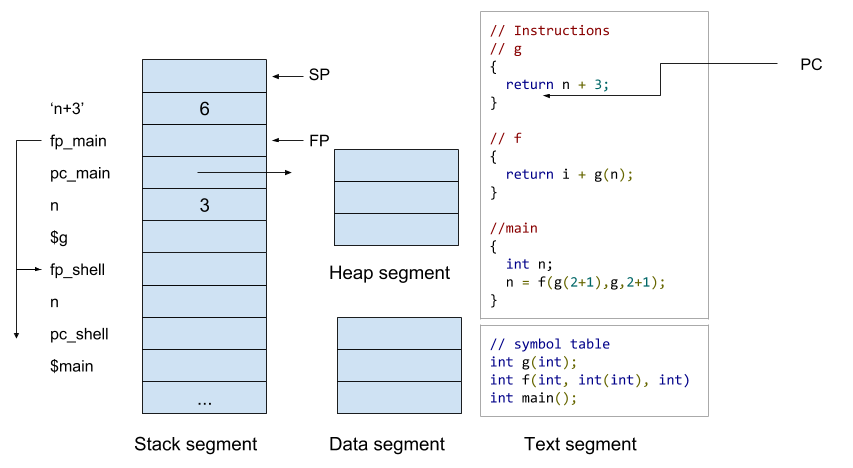
\includegraphics[width=0.9\textwidth]{figures/SOP_s05_ex1_a}
  \caption{\label{fig:ex1-a} Exercise 1-a.}
\end{figure}

\begin{figure}[ht]
  \centering
  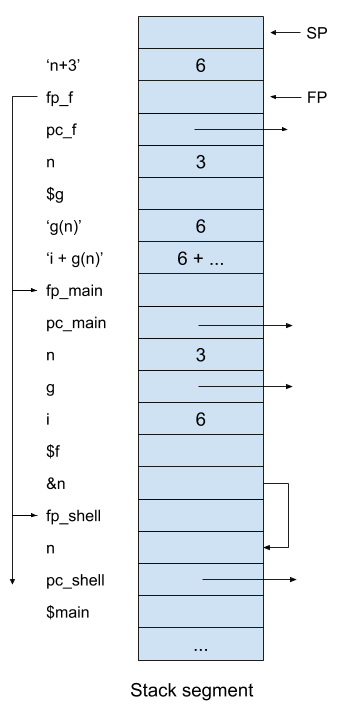
\includegraphics[width=0.4\textwidth]{figures/SOP_s05_ex1_b}
  \caption{\label{fig:ex1-a} Exercise 1-b.}
\end{figure}

\begin{figure}[ht]
  \centering
  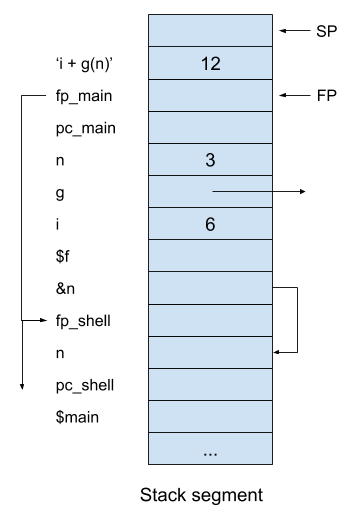
\includegraphics[width=0.4\textwidth]{figures/SOP_s05_ex1_c}
  \caption{\label{fig:ex1-a} Exercise 1-c.}
\end{figure}

\begin{figure}[ht]
  \centering
  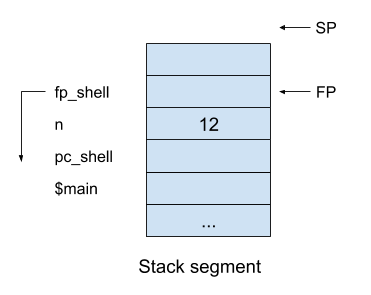
\includegraphics[width=0.4\textwidth]{figures/SOP_s05_ex1_d}
  \caption{\label{fig:ex1-a} Exercise 1-d.}
\end{figure}

\FloatBarrier

\section*{Exercise 2}

\subsection*{a)}

Figure~\ref{fig:ex2-a} shows the simplified stack segment for point A.

\begin{figure}[ht]
  \centering
  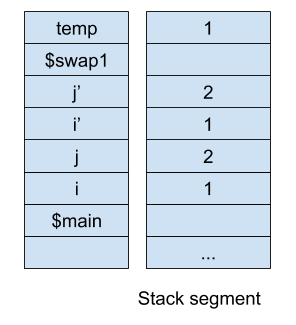
\includegraphics[width=0.4\textwidth]{figures/SOP_s05_ex2_a}
  \caption{\label{fig:ex2-a} Exercise 2-a.}
\end{figure}

\subsection*{b)}

Figure~\ref{fig:ex2-b} shows the simplified stack segment for point B.

\begin{figure}[ht]
  \centering
  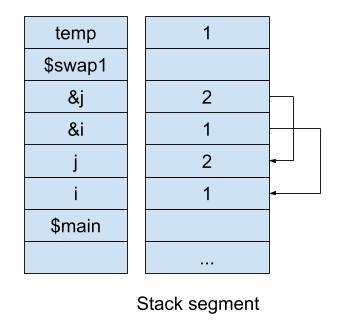
\includegraphics[width=0.4\textwidth]{figures/SOP_s05_ex2_b}
  \caption{\label{fig:ex2-b} Exercise 2-b.}
\end{figure}

\subsection*{c)}

Figure~\ref{fig:ex2-c} shows the diagram for point A.

\begin{figure}[ht]
  \centering
  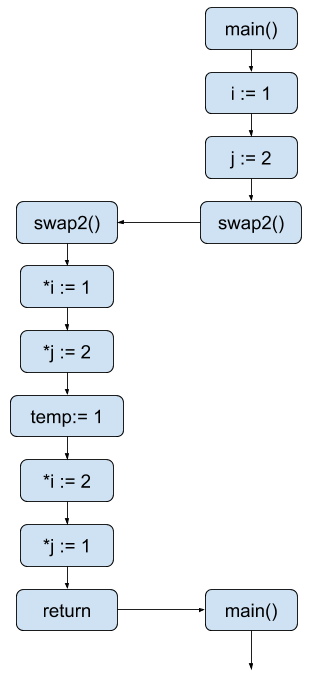
\includegraphics[width=0.3\textwidth]{figures/SOP_s05_ex2_c}
  \caption{\label{fig:ex2-c} Exercise 2-c.}
\end{figure}

We use the following list of gdb command :

\begin{verbatim}
// breakpoint at function swap2
br swap2
// breakpoint before returning from swap2
br 15
run

// display the variables
display i
display j
display temp

// display the arguments of stack2
frame 0

// continue to next breakpoint
c
// the value of i and j has been exchanged inside the function
n
// display the variables
display i
display j
// value have been exchanged
\end{verbatim}

\FloatBarrier

\section*{Exercise 3}

Figure~\ref{fig:ex3} show the stack and heap segment for a dynamic memory allocation.

\begin{figure}[ht]
  \centering
  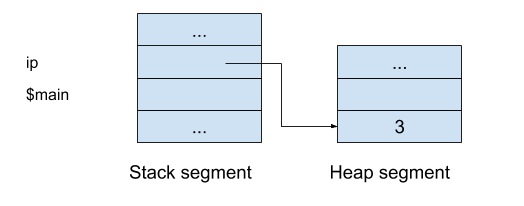
\includegraphics[width=0.6\textwidth]{figures/SOP_s05_ex3}
  \caption{\label{fig:ex3} Stack and heap segment for a dynamic memory allocation.}
\end{figure}

The casting is not necessary because a \cinline+void*+ is implicitely cast by
the compiler.

\section*{Exercise 4}

\subsection*{a)}

The ternary operator evaluates only one of the $2$ expressions depending on the
value of the logical expression in front of the $?$. So, if $bufp > 0$,
$getChar()$ is never call.

This buffer is like a cache memory because, when we $ungetch$ a character, we
don't discard it but push it in the buffer. So multiple alternate call to
$getch$ and $ungetch$ doesn't do any system call, which is clearly faster.

\subsection*{b)}

Here is the new implementation for $getop$ :

\begin{ccode}
int getop(char s[])
{
    static int buf[BUFSIZE];
    static int bufp = 0;

    char c;
    int i = 0;

    while ((c = (bufp > 0 ? buf[--bufp] : getchar())) == ' ' || c == '\t'); // skip spaces

    if (c < '0' || c > '9')                    // c is not a digit
        return c;

    s[0] = c;
    while (isdigit(s[++i] = c = (bufp > 0 ? buf[bufp--] : getchar())))    // collect integer
        ;
    s[i] = '\0';                               // string terminator
    // save the last read character
    if (c != EOF)
        if (bufp < BUFSIZE)
            buf[bufp++] = c;
        else
            printf("%d %d error\n", bufp, BUFSIZE);
    return NUMBER;
}
\end{ccode}

\subsection*{c)}

The variable are declared as static because they are ``private'' to the file. We
don't want the other files to know about our variables or allow them to interact
with our variables.

\subsection*{d)}

The header file are here in order to ``present'' the API of our modules. The
user of the file ``stack.h'', for example, don't have to know the exact details
of the implementation, just what the module offer is enough.

The files don't have to be protected by \verb+#ifndef+ because, when the
compiler is pre-processing the file, the \verb+include+ directives simply copy
paste the whole header file inside an another one. Multiple declaration of the
variable \verb+stack_error+ is not a problem as long as the type is the same.
For example, declaration as follow generate a compilation error :

\begin{ccode}
long stack_error;

int main(...)...
\end{ccode}

and a code like the following is accepted by the compiler :

\begin{ccode}
#include <stdio.h>
#include <stdlib.h>	// atof

#include "./stack/stack.h"  // push, pop
#include "./stack/stack.h"  // push, pop
#include "./getop/getop.h"  // GETOP_ERR, MAXOP, NUMBER, getop

int stack_error;

// reverse Polish calculator --- kr76
main()...
\end{ccode}

\end{document}
